\section{Theorie}
\label{sec:Theorie}
    Der Compton-Effekt beschreibt die Interaktion eines hochenergetischen Photons mit einem 
    niederenergetischen Elektron. Da das Elektron dabei Energie abgibt, verschiebt sich 
    die Frequenz des Photons in den höherfrequenten Raum. Diese Wellenlängendifferenz
    ist unabhängig von der ursprünglichen Wellenlänge und soll in diesem Versuch bestimmt 
    werden.\\
    \begin{figure}
        \centering
        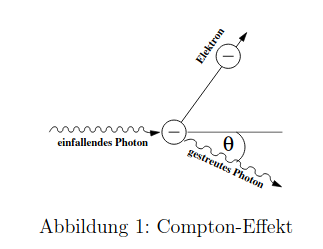
\includegraphics[width=\textwidth]{compton.png}
        \caption{Der Compton-Effekt}
        \label{fig:compost}
    \end{figure}
    Dazu wird Röntgenstrahlung erzeugt und an einem Plexiglasquader gestreut. Um die für 
    den Versuch relevante Röntgenstrahlung zu erzeugen, werden Elektronen aus einer 
    Glühkathode emmitiert und in einer evakuierten Röhre zu einer Anode beschleunigt. In der Anode
    entsteht durch das Abbremsen des Elektrons ein kontinuierliches Bremsspektrum. Außerdem 
    wird ein für das Anodenmaterial charakteristisches Spektrum ausgestrahlt, welches durch die 
    Ionisierung des Materials und das anschließende Rückfallen eines Elektrons auf eine weiter im 
    Zentrum liegende Schale entsteht. Dieses Spektrum besteht aus scharfen Peaks. \\
    \\
    Zu beachten ist, dass nicht nur Compton (kohärente) Streuung, sondern auch
    elastische (inkohärente) Streuung auf das Photon wirkt. Befindet sich das Elektron 
    vor dem Stoß in Ruhe, kann aus der Energie- und Impulserhaltung auf den Zusammenhang
    \begin{equation}
        \Delta \lambda = \dfrac{h}{m_e c}(1-\cos{\theta})=\lambda_c(1-\cos{\theta})
        \label{eqn:compt}
    \end{equation}
    geschlossen werden, wobei $\Delta \lambda$ die Wellenlängendifferenz, $\theta$ der 
    gestreute Winkel (siehe Abb.1), und $\lambda_c=h/(m_e c)$ die Compton-Wellenlänge ist.\\
    In dem Versuch wird Aluminium als Reflektions- und Transmissionsmaterial verwendet.
    Da die Transmission eines Körpers mit zunehmender Wellenlänge abnimmt, also die Transmission
    von Compton-gestreuter Photonen geringer ist, nimmt die Intesität des Lichts innerhalb eines 
    Körpers mit zunehmender Tiefe ab. Dieser Intesitätsverlust wird durch das Delamer'sche Gesetz
    \begin{equation}
        I = I_0 e^{-\mu d}
    \end{equation}
    beschrieben. Dabei stellt $\mu$ den Absorptionskoeffizienten dar, der sich aus dem 
    Absorptionskoeffizienten für Paarbildung, des Photoeffektes und des Comptoneffektes 
    zusammensetzt.\\
    Um die resultierende Wellenlänge zu bestimmen, wird auf einen LiF-Kristall und die Bragg'sche Bedingung
    \begin{equation}
        2 \ d \sin{\alpha} = n\lambda
        \label{eqn:bragg}
    \end{equation}
    mit Einfallswinkel $\alpha$, Gitterkonstante d und Beugungsordnung n, zurückgegriffen.
    Diese tritt bei Kristallen auf, in denen Atome bekanntermaßen in Gitterstrukturen 
    angelegt sind und resultiert aus der Interferenz von durch verschiedene Gitterebenen 
    reflektierte Photonen.

